
\documentclass{article}
\usepackage{amsmath, amsfonts, amssymb, amsthm} %packages for math-related
\usepackage[margin=1.2in]{geometry}
\usepackage[shortlabels]{enumitem}
\usepackage[utf8]{inputenc}
\usepackage{graphicx} % package for inserting images
\usepackage{commath} % package for things like \del, \cbr, and \sbr. These handle parentheses well.
\usepackage[mathscr]{euscript}%for \scr command 
\usepackage{../commands} %package with all of the commands for this class
\usepackage{url}
\setlength{\parindent}{0em} % so paragraphs aren't indented
\newcommand{\lcm}{\text{lcm}}
\newcommand{\Hom}{\text{Hom}}
\newcommand{\Ann}{\text{Ann}}

% ********************************************************** %
%               THINGS TO EDIT BELOW THIS LINE               %
% ********************************************************** %
\newcommand{\D}{\nabla}
\renewcommand{\d}{\partial}

\title{\textsc{MATH 173 Problem Set 1}}
\author{Stepan (Styopa) Zharkov}
\date{April 6, 2022}
\begin{document}
\maketitle
\problem{1} Let $f \in C^2(\RR^3)$. Define $F = \D f$ . Show that $\D \times F = 0$ and that $\D \cdot F = \Delta f$. \tri
\hop
\solution
First, we see that 
\[\D \times F = \D \times \D f = \del{\d_2\d_3 f - \d_3\d_2 f,\d_3\d_1 f - \d_3\d_1 f, \d_1\d_2 f - \d_1\d_2 f} = (0,0,0)\]
because order of differentiation does not matter. Also, 
\[\D \cdot F = \D \cdot \D f = \d_1\d_1 f +  \d_2\d_2 f  + \d_3\d_3 f  = \Delta f,\]
as we wanted. \qed


\newpage
\problem{2}Consider the following first order linear equation with constant coefficients
$\d_1u + \d_2u = 0$, where $u = u(x_1, x_2) : \RR^2 \to \RR$.
\begin{enumerate}[(a)]
    \item Give an example of a non-zero solution with satisfies $u(x, x) = 0$ for all $x \in \RR$.
    \item Show that if $u$ solves the equation and satisfies $u(x, -x) = 0$ for all $x$, then $u = 0$.
    \item Describe all solutions $u \in C^1(\RR^2)$.
\end{enumerate}
\tri
\hop
\solution 
\begin{enumerate}[(a)]
    \item Consider $u(x_1, x_2) = x_1 - x_2$. We see that $\d_1u+\d_2u=1-1=0$ and $u(x,x)=0$, but $u$ is nonzero.\qed
    \item Suppose $u(\hat x_1, \hat x_2) \ne 0$ for some $\hat x_1, \hat x_2$. Consider the function $f(s) = u(\hat x_1 + s, \hat x_2 + s)$. We see that $f(0)\ne 0$ and $f((-\hat x_1 -\hat x_2)/2)= u((\hat x_1-\hat x_2)/2, (-\hat x_1+\hat x_2)/2) = 0$. By the mean value theorem, there is some point where $f' \ne 0$. 
    \hop
    However, we see that $f'(s) = \d_1u(\hat x_1+s,\hat x_2+s)+\d_2u(\hat x_1+s, \hat x_2+s) = 0$. So, we have a contradiction and thus there is no such $\hat x_1, \hat x_2$ and $u = 0$. \qed
    \item Let $f_r(s) = u(r+s,-r+s)$. We $f'(s) = \d_1u(r+s,-r+s)+\d_2u(r+s, -r+s) = 0$, so $f_r$ is constant. Thus, $u(r,-r)$ defines all of $f_r$. Note that any point $(x_1, x_2)$ is expressed uniquely as $(r+s, -r+s)$, so the $f_r$ cover the entire plane with no overlap. 
    \hop
    In other words, Any solution can be described as $u(x_1, x_2) = g((x_1-x_2)/2)$ where $g(r): \RR \to \RR$ is a $C^1$ function. We also see that any choice of $g$ gives a solution, so this characterizes all solutions. \qed
\end{enumerate}

\begin{center}
    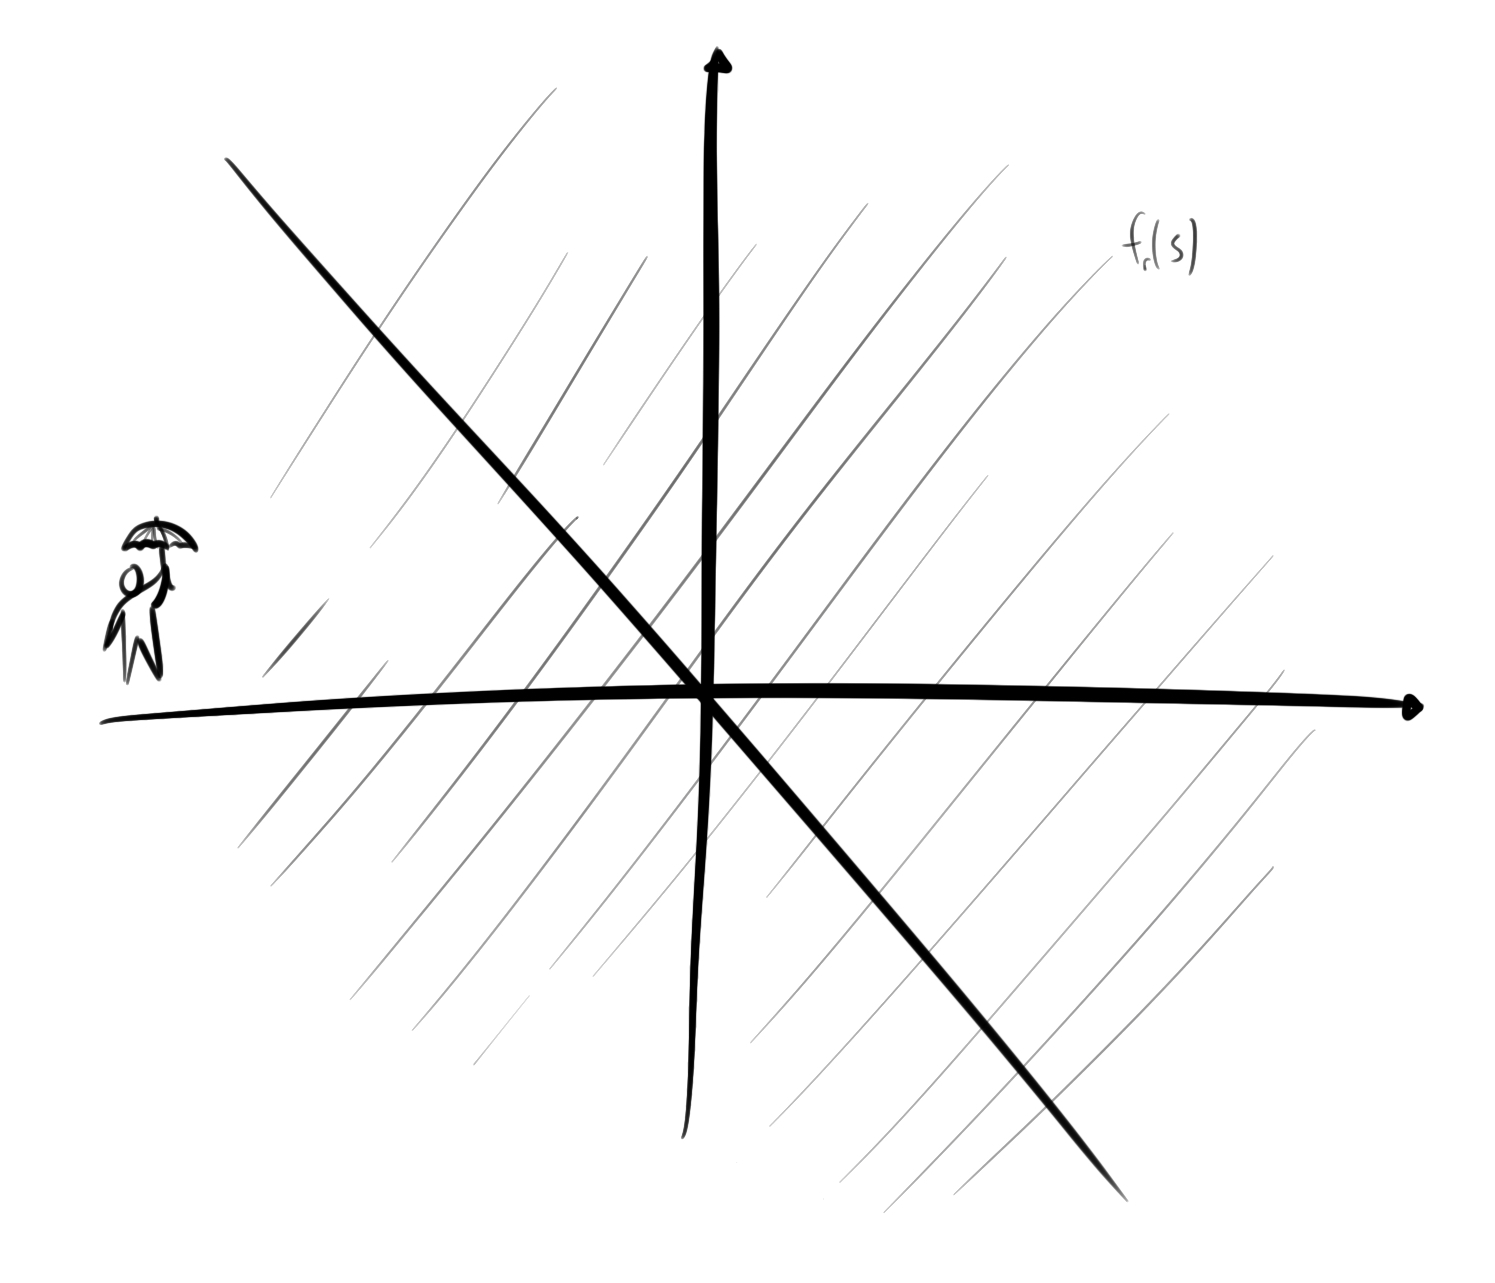
\includegraphics[height=6cm]{../images/rain}
\end{center}

\newpage
\problem{3} Let $p > 0$, the equation $\D \cdot (|\D u|^{p-2}\D u) = 0$ is called the $p$-Laplace equation.
\begin{enumerate}[(a)]
    \item Rewrite the equation to show that it is quasilinear.
    \item Find the Euler-Lagrange equation for the functional $I(u) = \int_D F (x, u, \d u)dx$, where
    $F (x, y, v) = |v|^p =
    \del{\sum^n
    _{j=1} v^2_j
    }^{p/2}$
    . Compare to the $p$-Laplace equation.
\end{enumerate}\tri
\hop
\solution
\begin{enumerate}[(a)]
    \item This problem is solved by bashing. We see that 
    \begin{align*}
        \D \cdot \del{\abs{\D u}^{p-2}\D u} &=\sum_{i=1}^n \frac{\d}{\d x_i} \del{\abs{\D u}^{p-2}\frac{\d u}{\d x_i}} \\ 
        &= \sum_{i=1}^n \del{\frac{\d u}{\d x_i}\frac{\d}{\d x_i}\abs{\D u}^{p-2}}+\sum_{i=1}^n\abs{\D u}^{p-2}\frac{\d^2u}{\d x_i^2}\\
        &= \sum_{i=1}^n \del{\frac{\d u}{\d x_i}\frac{\d}{\d x_i}\abs{\D u}^{p-2}}+\abs{\D u}^{p-2}\Delta u.
    \end{align*}
    Now, we can check that 
    \begin{align*}
        \frac{\d}{\d x_j}\abs{\D u}^{p-2} &= \abs{\D u}^{p-3}(p-2)\frac{\d}{\d x_j} \del{\sum_{i=1}^n \del{\frac{\d u}{\d x_i}}^2}^{1/2} \\
        &= \abs{\D u}^{p-4} (p-2) \sum_{i=1}^n \frac{\d u }{\d x_i}\frac{\d^2 u}{\d x_i x_j}. 
    \end{align*}
    Plugging this in to our first computation, we see that 
    \begin{align*}
        \D \cdot \del{\abs{\D u}^{p-2}\D u} =  \abs{\D u}^{p-4}(p-2) \sum_{j=1}^n \sum_{i=1}^n \del{\frac{\d u}{\d x_j}\frac{\d u }{\d x_i}\frac{\d^2 u}{\d x_i x_j}}+\abs{\D u}^{p-2}\Delta u.
    \end{align*}
    We see that $\abs{\D u}^{p-2}$ and $\abs{\D u}^{p-4}$ are functions of the first partial derivatives of $u$, and $\Delta u$ is a linear function of second derivatives, so this is indeed in the quasilinear form 
    \[\sum_{|\alpha|=2}a_\alpha(x,u,\d u)(\d^\alpha u)\]
    and our expression is quasilinear. \qed
    \item This problem is also manipulations. First, note that for $F(x,y,v) = |v|^p$, we have $\d_y F=0$ and $\d_{x_j} F =0$. So.in the general form of the Euler-Lagrange equation, most terms are 0 and we are left with 
    \[\sum_{j=1}^n\sum_{k=1}^n \d_{v_k}\d_{v_j}|v|^p \d_k\d_j u = 0.\]
    We can see that 
    \[\d_{v_j} |v|^p = \d_{v_j}\del{\sum_{i=1}^n v_i^2}^{p/2} = pv_j \del{\sum_{i=1}^n v_i^2}^{p/2-1}.\]
    Continuing with the computation, we see that for $j \ne k$
    \[\d_{v_k}\d_{v_j} |v|^{p} = v_kv_jp(p-2)\del{\sum_{i=1}^n v_i^2}^{p/2-2}\]
    and for $j =k$, 
    \[\d_{v_k}\d_{v_j} |v|^{p} = v_kv_jp(p-2)\del{\sum_{i=1}^n v_i^2}^{p/2-2} + p\del{\sum_{i=1}^n v_i^2}^{p/2-1}.\]
    Placing this in the original equation, we have 
    \begin{align*}
        0 &= \sum_{j=1}^n\sum_{k=1}^n \d_{v_k}\d_{v_j}|du|^p \d_k\d_j u \\
        &= p \sum_{j,k =1}^n \del{ (\d_k u)(\d_j u)(p-2)\del{\sum_{i=1}^n (\d_i u)^2}^{p/2-2}\d_j\d_k u} + p\sum_{j=1}^n\del{\del{\sum_{i=1}^n (\d_iu)^2}^{p/2-1}\d_j\d_j u} \\
        &= p\del{(p-2)\abs{\D u}^{p-4}\sum_{j,k = 1}^n\del{(\d_j u)(\d_k u)\d_j\d_k u} + \abs{\D u}^{p-2}\sum_{j=1}^n(\d_j\d_j u)}\\
        &= p\del{\D \cdot \del{\abs{\D u}^{p-2}u}}
    \end{align*}
    by part (a). Since $p>0$, we can divide both sides by $p$ to get 
    \[0 = \del{\D \cdot \del{\abs{\D u}^{p-2}u}},\]
    which is precisely the $p$-Laplace equation. \qed
\end{enumerate}


\newpage
\problem{4} Solve the equation $x_1\d_1u+x_2\d_2u+(x_1-1)u = 0$ with the condition $u(x, e^x) = x$.
In which region is $u$ uniquely determined?\tri
\hop
\solution We can rewrite the equation as 
\[x_1\d_1u+x_2\d_2u=(2-x_1)u\]
First, let's find the characteristic curves with starts on the curve $\Gamma: x_2 = e^{x_1}$. Any characteristic curve $f$ has $f_1'(s) = s$ and $f'_2(s) = s$ with $f_2(0)=e^{f_1(0)}$. 
\hop 
Solving this, we have $f_1(s) = re^s$ and $f_2(s) = e^re^s$ for some $r$. Let $f_r(s) = (re^s, e^re^s)$ be the characteristic curves, then. Since $e^s$ can be any positive number and the vector $(r,e^r)$ can point in any direction above the $x_1$-axis and above the line of slope $e$, we see that our characteristic curves cover the plane above these two lines.
\hop
Let $y_r(s) = u(f_r(s))$. Since $f_r$ are characteristic curves, we know $y_r'(s)=(2-re^s)$ and $y_r(0)=re^0 = r$. Using our calculus methods, we have $dy/y = (2-re^s)ds$, so $\ln y = 2s-re^s+c$. The initial condition gives us that  
\[y_r(s)=e^{2s-re^s+r+\ln r}=re^{2s-re^s+r}.\]
Since we can express $x_1 = re^s$ and $x_2 = e^{r+s}$, we see that 
\[u(x_1,x_2) = y_r(s) = re^{2s-re^s+r} = re^s \cdot e^{s+r}\cdot e^{-re^s} = x_1x_2e^{-x_1}\]
for all points $(x_1, x_2)$ that are on some characteristic curve. We can confirm the solution by differentiating. So, we have found a solution $u$ that is locally determined on the region above the $x_1$-axis and the line with slope $e$. \qed
\begin{center}
    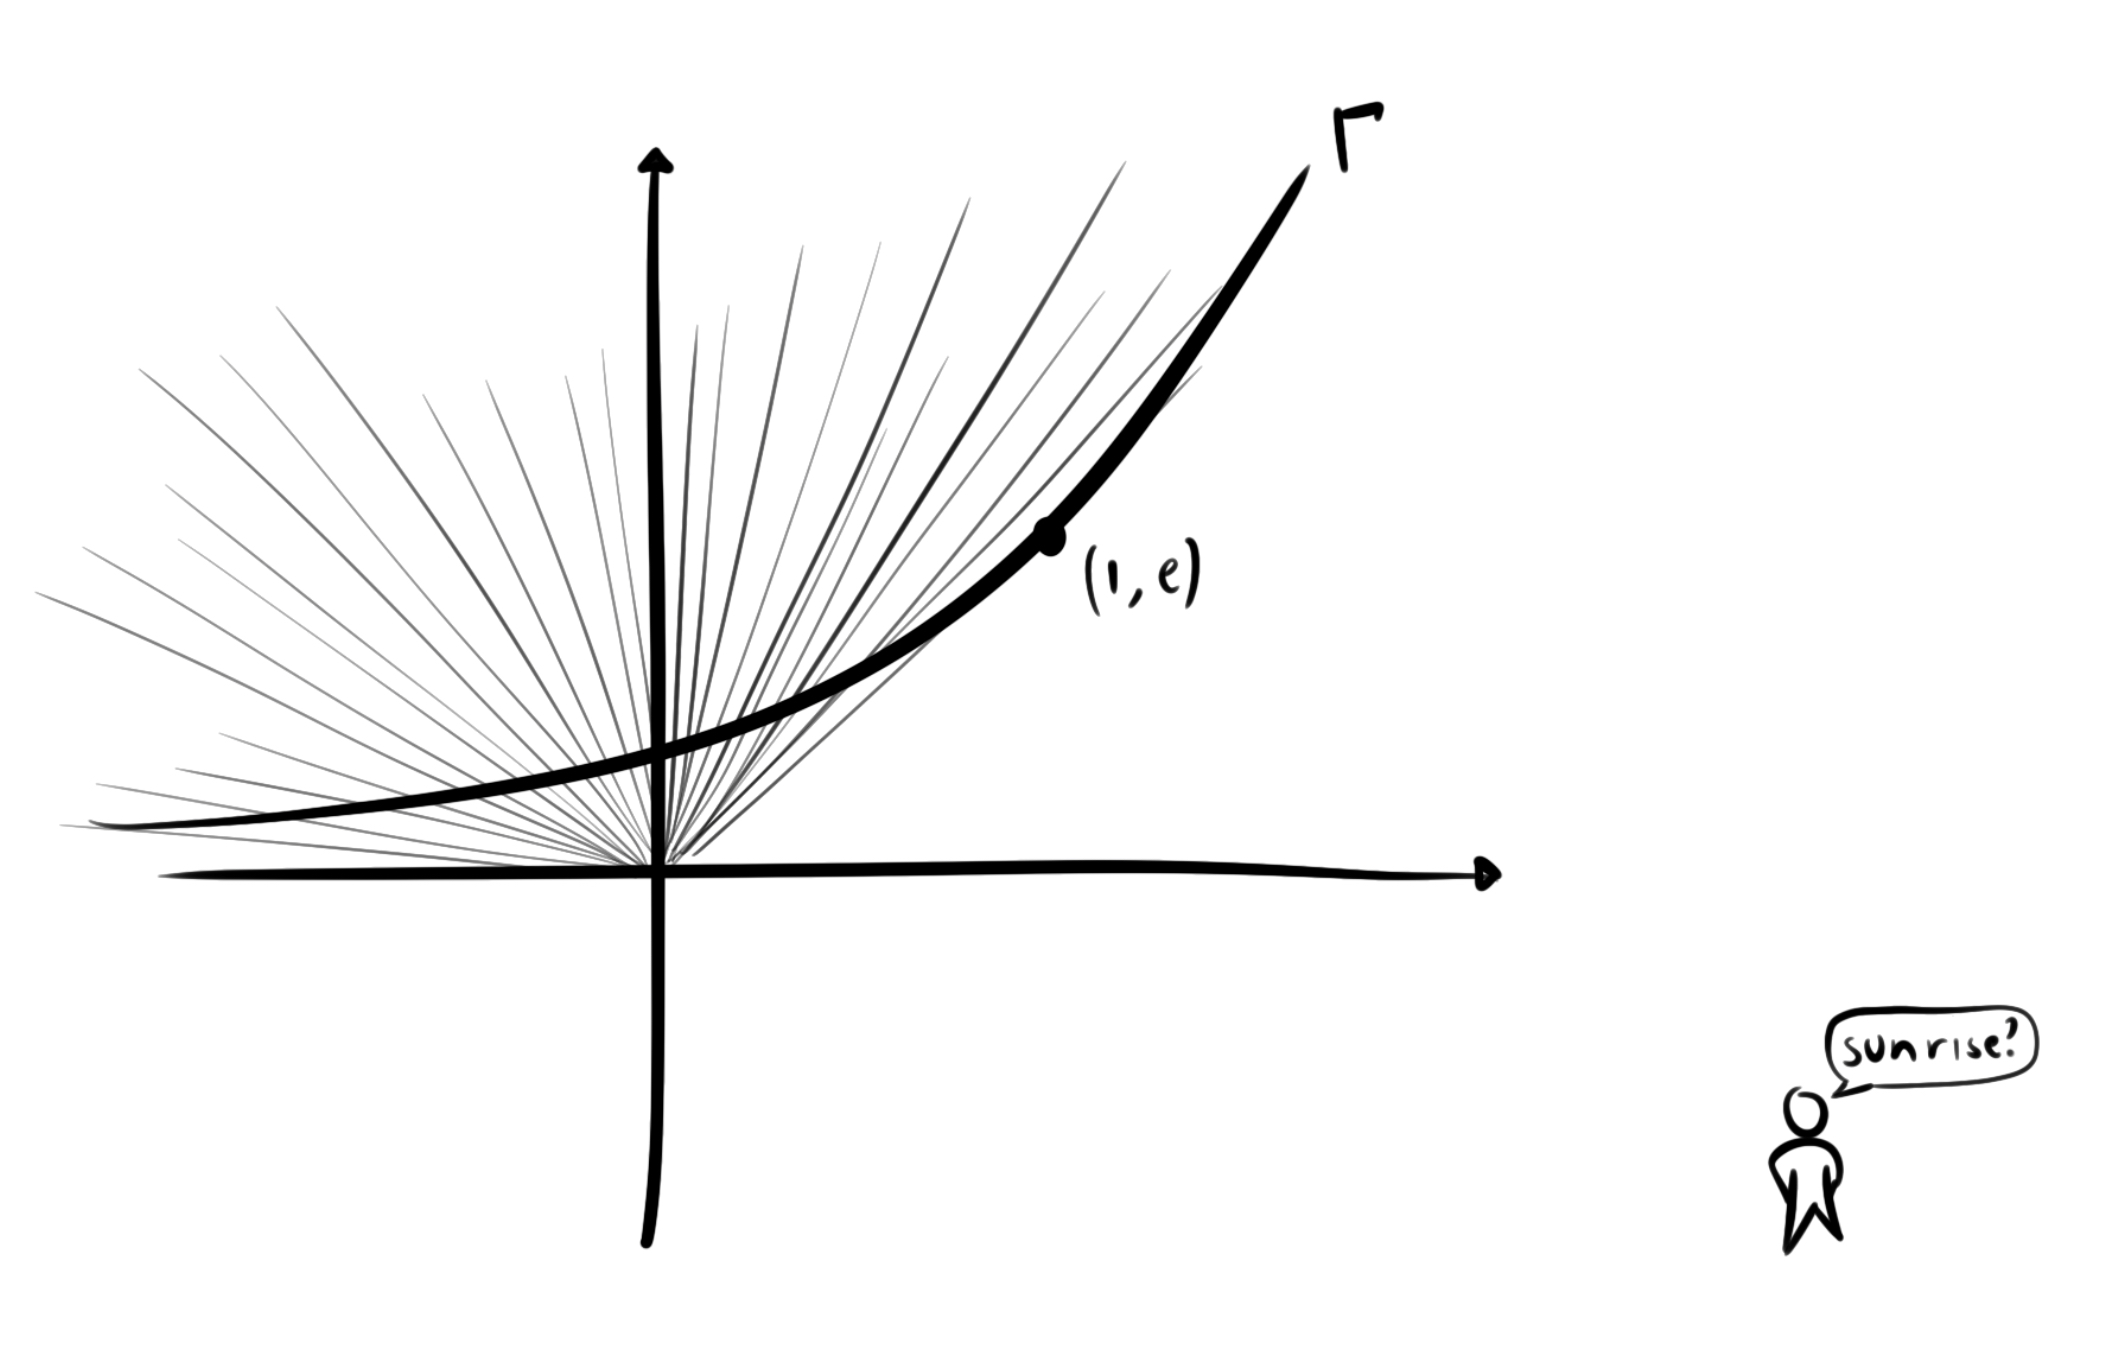
\includegraphics[height=6cm]{../images/sunrise}
\end{center}
\newpage
\problem{5} 
\begin{enumerate}[(a)]
    \item Solve the equation $x_1\d_1u+x_2\d_2u+x_1x_2\d_3u = 0$ with the condition $u(x1, x2, 0) =
    x^2_1 + x^2_2$.
    \item Compute $u(1, 1, 1)$ for the solution in part (a). Explain why $u(1, 1, 1)$ is negative while the
    initial condition is non-negative.
\end{enumerate}
\tri
\hop
\solution
\begin{enumerate}[(a)]
    \item This problem is solved using the same idea as problem 4, but with three variables. First, let's find the characteristic curves starting on the surface $\Gamma: x_3 = 0$. 
    Any characteristic curve $f$ has $f_1'(s) = f_1(s)$, $f_2'(s) = f_2(s)$, and $f_3'(s) = f_1(s)f_2(s)$ with $f_3(0) = 0$. 
    \hop 
    Solving this, we have $f_1(s) = ae^s$, $f_2(s)=be^s$, and $f_3(s)=\frac{1}{2}abe^{2s}-\frac{1}{2}ab$. So, let 
    \[f_{a,b}(s) = \del{ae^s, be^s,\frac{1}{2}abe^{2s}-\frac{1}{2}ab}\]
    be the characteristic curves. Now, along the curve $f_{a,b}$, we can define $y_{a,b}(s) = u(f_{a,b}(s))$ and we know $y'_{a,b}(s) = 0$ as well as $y_{a,b}(0) = f_1(0)^2 + f_2(0)^2 = a^2+b^2$. So, $y_{a,b}$ is the constant function with a value of $a^2 + b^2$. 
    \hop 
    We can write $x_1 = ae^s$, $x_2 = be^s$ and $x_3=\frac{1}{2}abe^{2s}-\frac{1}{2}ab$. So,
    \[s = \frac{1}{2}\ln\del{\frac{\frac{1}{2}x_1x_2}{\frac{1}{2}x_1x_2-x_3}}, a = \frac{x_1}{\sqrt{\frac{\frac{1}{2}x_1x_2}{\frac{1}{2}x_1x_2-x_3}}}, b = \frac{x_2}{\sqrt{\frac{\frac{1}{2}x_1x_2}{\frac{1}{2}x_1x_2-x_3}}}\]
    for all $x_1,x_2,x_3$ such that 
    \[\frac{\frac{1}{2}x_1x_2}{\frac{1}{2}x_1x_2-x_3} > 0.\]
    Plugging this in, we have that 
    \[u(x_1, x_2, x_3) = y_{a,b}(s)=a^2+b^2 = \frac{x_1^2 + x_2^2}{\frac{\frac{1}{2}x_1x_2}{\frac{1}{2}x_1x_2-x_3}} = \frac{(x_1^2+x_2^2)(x_1x_2-2x_3)}{x_1x_2}\]
    for all such $x_1, x_2,x_3$. We can confirm the solution by differentiating. So, we have solved the equation on part of the space. \qed
    \item We see that $u(1,1,1) = -2$ even though initial conditions are non-negative and $u$ is constant along any characteristic curve. This is possible because the point $(1,1,1)$ is not within the boundary of where our solution works. No characteristic curve goes through $(1,1,1)$. We needed
    \[\frac{\frac{1}{2}x_1x_2}{\frac{1}{2}x_1x_2-x_3} > 0\]
    and this isn't true for $(1,1,1)$. \qed
\end{enumerate}

\newpage
\problem{6} Find general solution to the equation $x_1\d_1u + ... + x_n\d_nu = cu$. \tri
\hop
\solution Let $\Gamma$ be the unit sphere $\SS^{n-1}$. Let $u$ restricted to the unit sphere be $g: \SS^{n-1} \to \RR$. If $f$ is a characteristic curve with a start on $\Gamma$, then $f_i'(s) = f_i(s)$, so $f_i(s) = a_ie^s$ and we can define
\[f_a(s)=(a_ie^s, \dots, a_ne^s)\]
as the characteristic curve, where $a = (a_1, \dots, a_n) \in \SS^{n-1}$. Intuitively, these are rays pointing out of the origin. Let $y_a(s)=u(f_a(s))$. We see that $y'_a(s) = cy_a(s)$ and $y_a(0) = g(a)$, so $y_a(s) = g(a)e^{cs}$. 
\hop
Note that we can place any nonzero $x \in \RR^n$ on a characteristic curve uniquely with $a = \frac{x}{|x|}$ and $e^s = |x|$. So, we can write 
\[u(x) = y_a(s) = g(a)e^{cs} = g\del{\frac{x}{|x|}}|x|^c\]
as the general solution defined everywhere but the origin, where $g$ is some $C^1$ function on the sphere. \qed

\begin{center}
    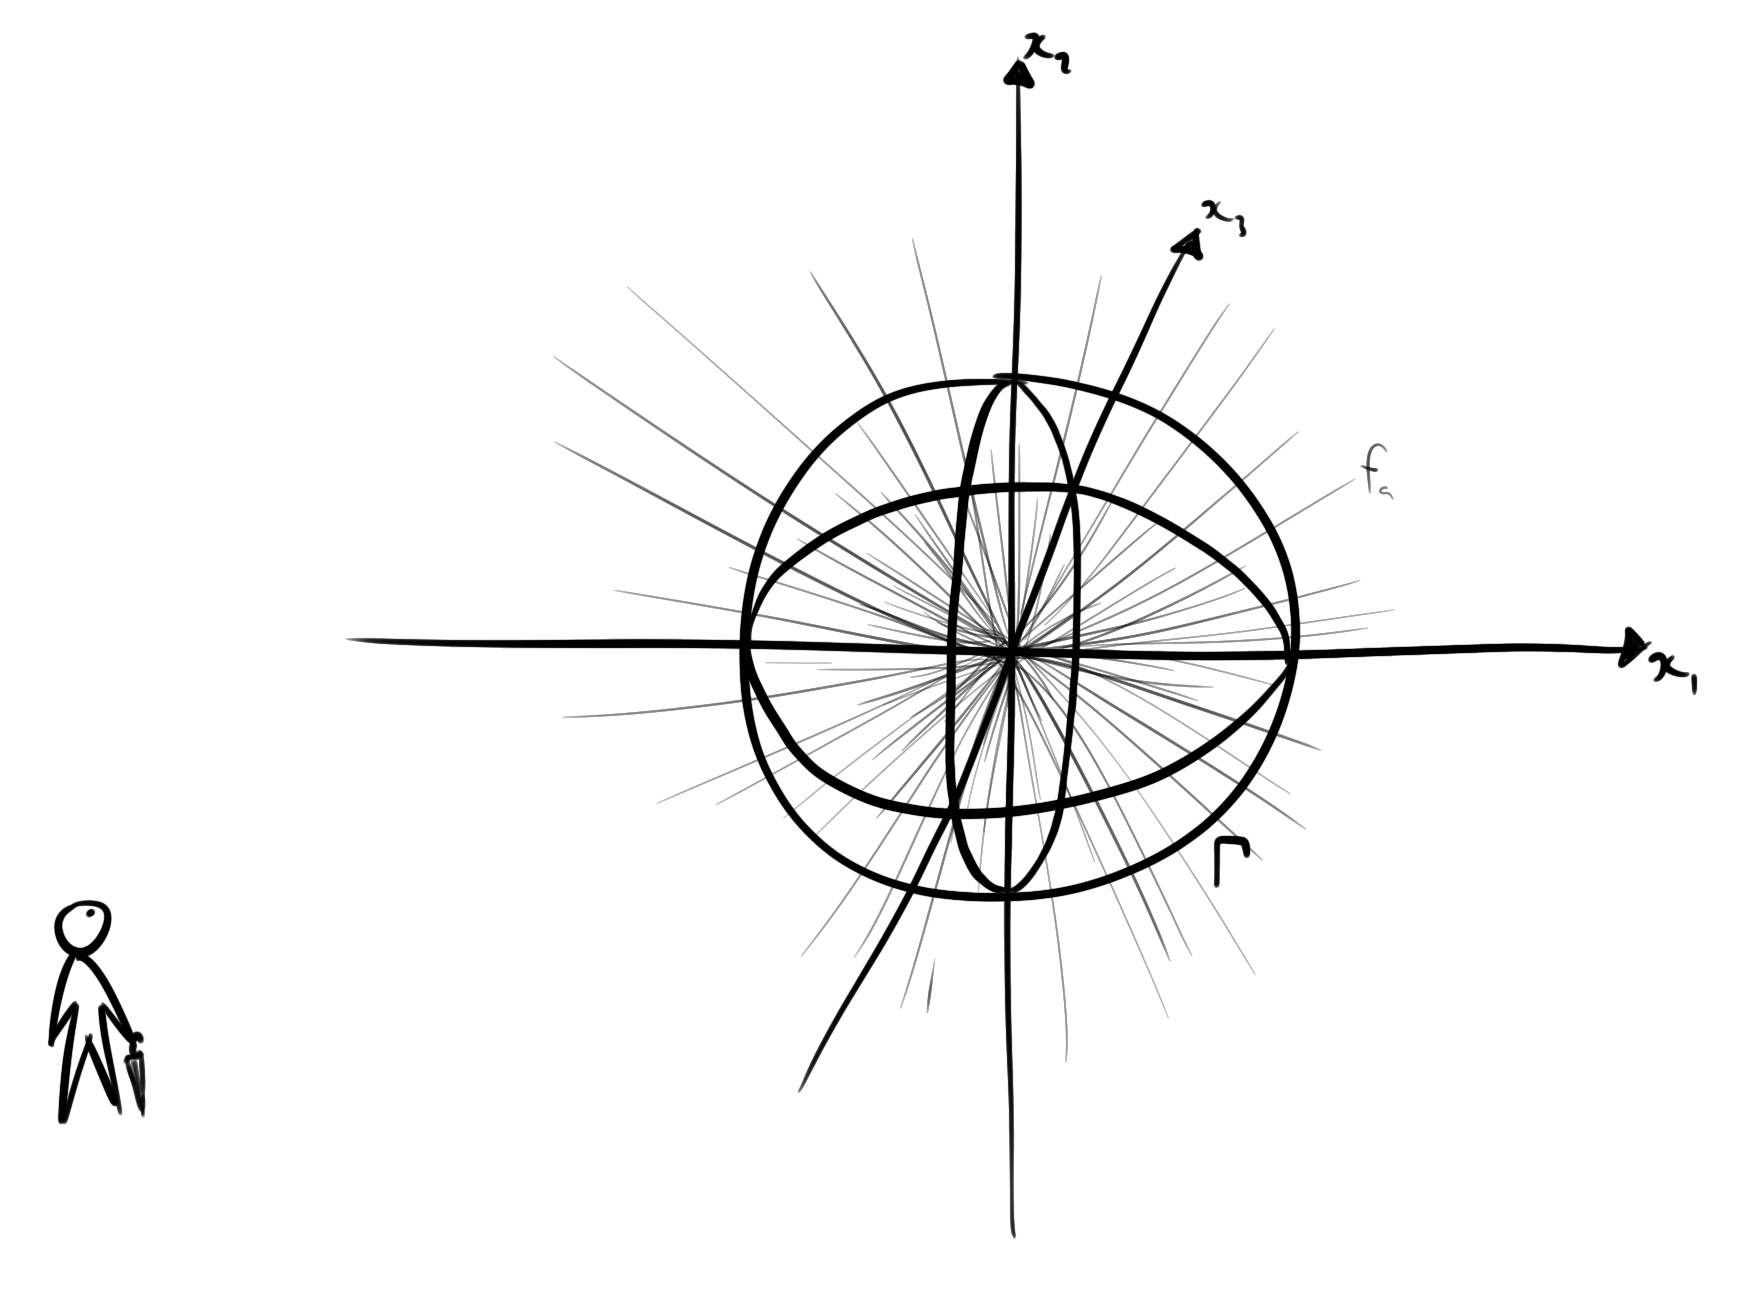
\includegraphics[height=6cm]{../images/explosion.jpeg}
\end{center}


\newpage
\problem{7} 
\begin{enumerate}[(a)]
    \item Solve $u_t + u_x = u^2, u(0, x) = e^{-x^2}$.
    \item Show that there is $T > 0$ such that $u$ blows up at time $T$ , i.e. $u$ is continuously differentiable
    for $t \in [0, T )$, and $x$ arbitrary, but for some $x_0, \lim_{t\to T^-}|u(x_0, t)|= \infty$. What is $T$ ?
\end{enumerate}
\tri
\hop
\solution
\begin{enumerate}[(a)]
    \item This problem is solved similar to problem 4 and 5. First, let's find the characteristic curves starting on the surface $\Gamma: t = 0$. We see that if $f$ is a characteristic curve, then $f_t'(s) = 1$, $f_x(s)' =1$ and $f_t(0)= 0$.
    \hop
    Solving this, we have $f_t(s) = s$ and $f_x(s) = s+r$. So, we can let
    \[f_r(s)=(s, s+r)\]
    be the characteristic curves. We can define $y_r(s) = u(f_r(s))$ along the curves, and we know $y_r'(s) = y_r(s)^2$ with $y_r(0) = e^{-f_x(0)^2} = e^{-r^2}$. 
    \hop
    We can solve for $y$ in the exact same way as Example 3.3 in the lecture notes to get that 
    \[y_r(s) = \frac{1}{e^{r^2}-s}\]
    when $s \ne e^{r^2}$. Since we can write $s = t, r = x-t$, we see that 
    \[u(x,t) = \frac{1}{e^{(x-t)^2}-t}\]
    when $e^{(x-t)^2} \ne t$. So, we have a solution that blows up on the curve $e^{(x-t)^2} = t$. \qed

    \begin{center}
        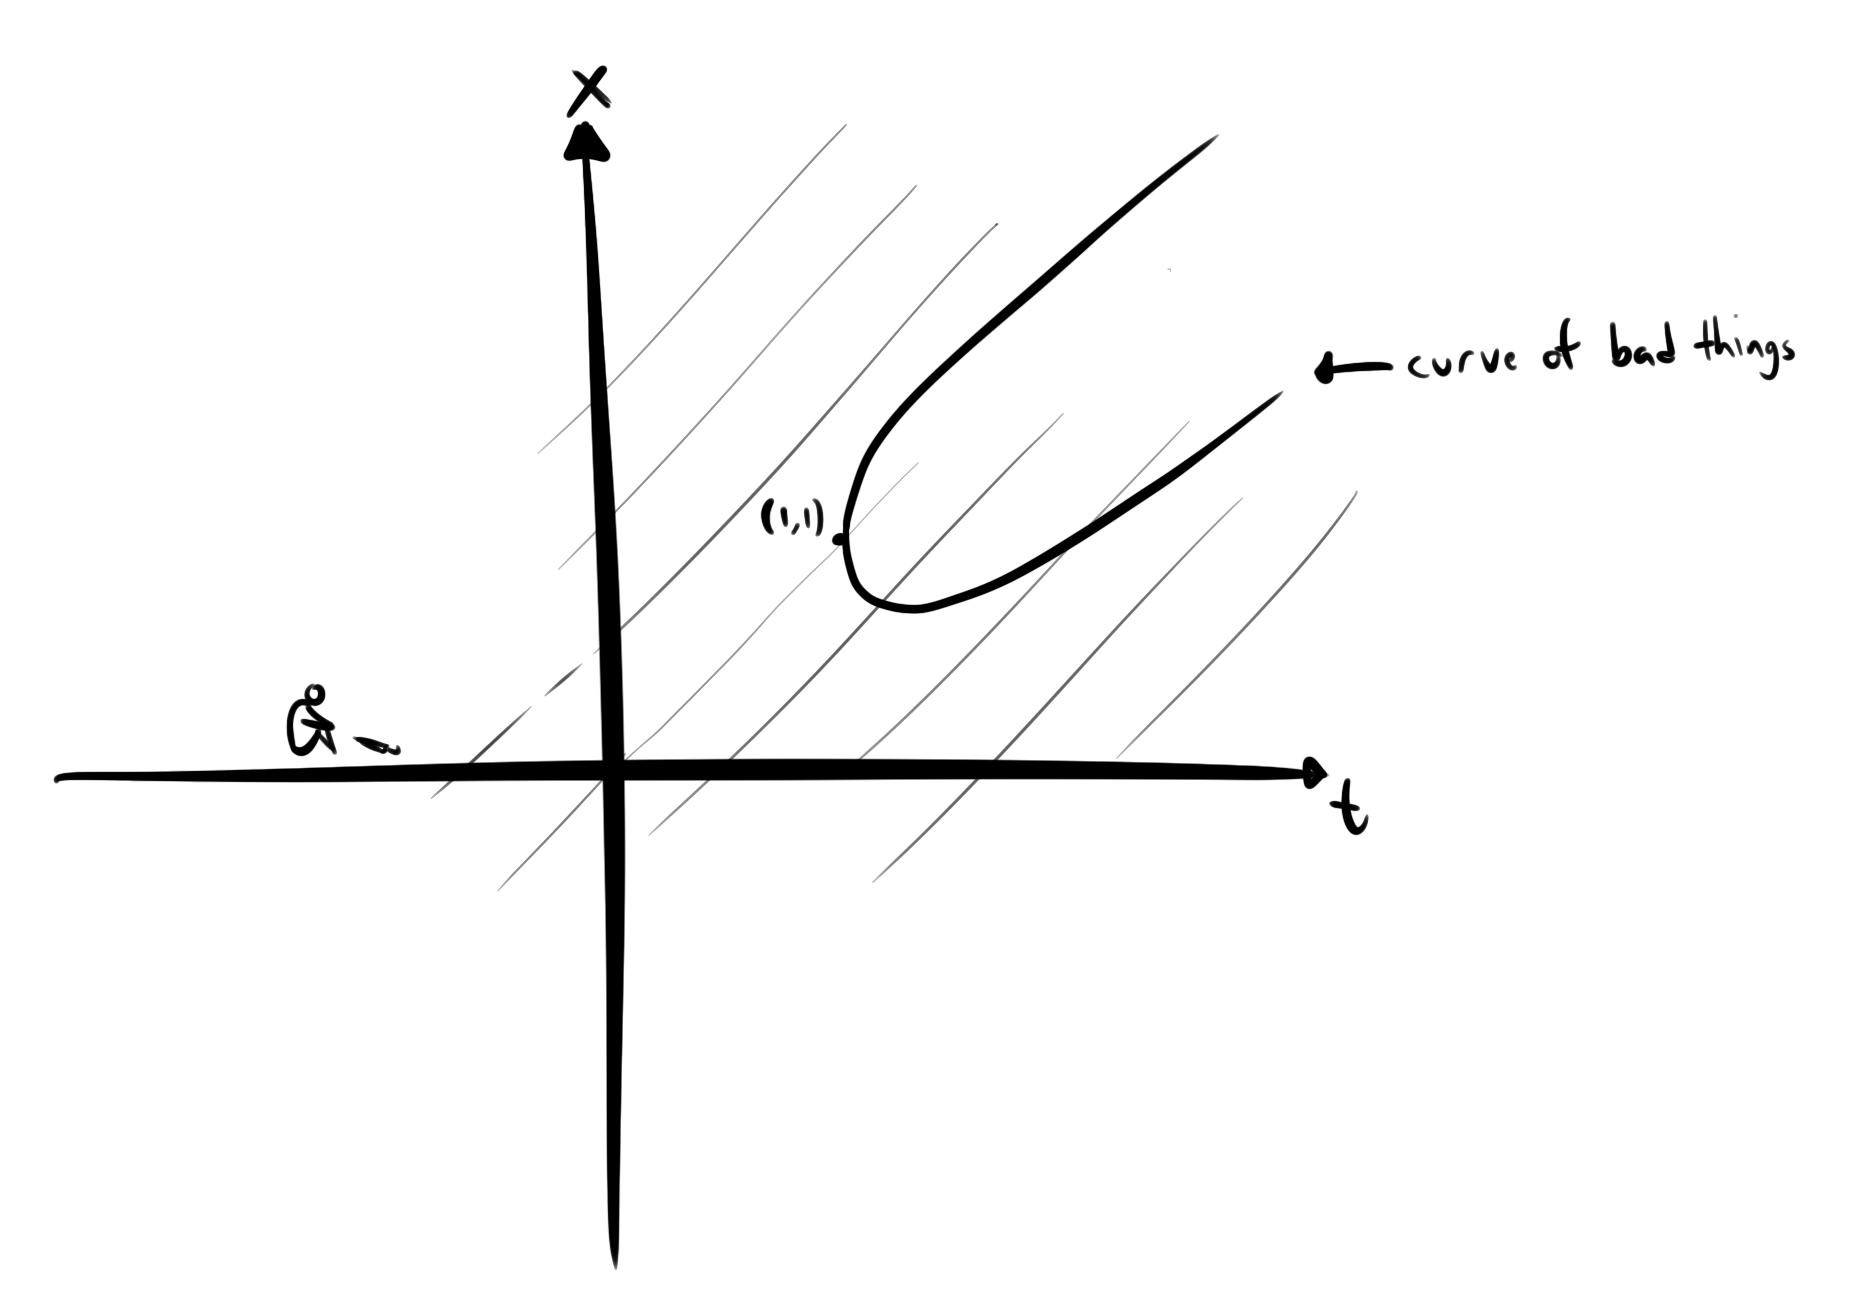
\includegraphics[height=6cm]{../images/comet}
    \end{center}

    \item The intuition for this problem is that we must pick a $T$ such that the vertical line of $t = T$ just barely touches the blow up curve in the picture above.
    \hop
    Let $T=1, x_0 = 1$. We see that for $t < T$, we have $e^{(x-t)^2} \ge 1 > t$,  so $\frac{1}{e^{(x-t)^2}-t} = u(x,t)$ is continuously differentiable. However, 
    \[\lim_{t \to 1^-}\frac{1}{e^{(1-t)^2}-t} = \infty\]
    because both $e^{(1-t)^2}$ and $t$ approach 1 as $t \to 1^-$. So, we have found the desired point. \qed
\end{enumerate}

\end{document}